\vspace*{-1cm}

\nombreCapituloCabecera{RH}{Análisis} % Título de la sección en la cabecera

\section{Análisis} % Título del capítulo
\label{sec:analisis}

% ---------------------------------------------------


\subsection{Especificación de requisitos}
En un escenario habitual, se deberán especificar, al menos, los siguientes tipos de requisitos:

\begin{itemize}
    \item Funcionalidades del sistema, que podrán detallarse, por ejemplo, mediante diagramas de casos de uso con su especificación. Alternativamente se pueden mostrar historias de usuario.
    \item Interfaz de usuario (si procede). Puede incluirse, por ejemplo, el nivel de cumplimiento de la norma de accesibilidad WCAG.
    \item Rendimiento (si procede), incluyendo tiempos de respuesta.
    \item Capacidad (si procede), incluyendo el número máximo de peticiones que se pueden procesar por unidad de tiempo.
    \item Seguridad (si procede). Se indicará el nivel de seguridad que ha de satisfacer el sistema, por ejemplo, según el Esquema Nacional de Seguridad (RD 3/2010) o según alguna norma de la familia ISO 27000. Este nivel de seguridad se establecerá a partir de un análisis de riesgos (véase la sección de análisis de seguridad).
    \item Interoperabilidad con otros sistemas (si procede).
    \item Protección de datos (si procede), en concreto, el cumplimiento del Reglamento General de Protección de Datos ([UE] 2016/679) y de la Ley Orgánica 3/2018 de Protección de Datos Personales y Garantía de los Derechos Digitales (véase la sección de análisis desde la perspectiva del RGPD).
    \item Requisitos sobre entorno tecnológico y de comunicaciones (si procede), es decir, requisitos sobre gestores de bases de datos, sistema o los sistemas operativos, hardware, protocolos de red, etc.
\end{itemize}


\begin{table}[h]
    \centering
    % chktex-disable 44

        \captionazul{Ejemplo ilustrativo de una tabla}

        \setlength{\arrayrulewidth}{0.05mm} % <--- Grosor más fino (el estándar es 0.4pt)
        \begin{tabular}{|p{2cm}|p{10cm}|}
            \hline
            \textbf{Ref.} & \textbf{Descripción} \\
            \hline
            RF01 & Descripción del requisito funcional 01. \\
            \hline
            RF02 & Descripción del requisito funcional 02. \\
            \hline
            \ldots & \ldots \\
            \hline
            RFN & Descripción del requisito funcional N. \\
            \hline
        \end{tabular}
    \label{tab:requisitos_funcionales}
\end{table}

\subsection{Análisis de los Casos de Uso}

Deberán identificarse los diferentes casos de uso del sistema. Podrá elaborarse un Diagrama de Casos de Uso y/o Diagrama de Contexto del sistema. Si es necesario elaborar varios diagramas de casos de uso, en esta sección se incluirán sólo los más relevantes. El resto se podrán incluir en un anexo.

\begin{figure}[H]
    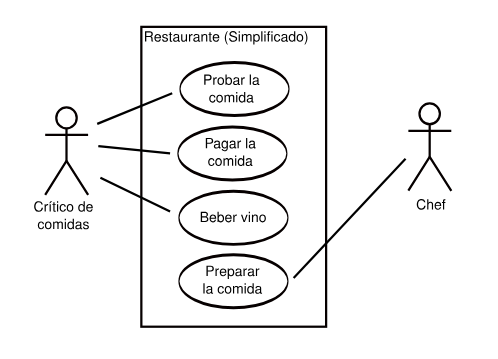
\includegraphics{Imagenes/Imagen-ejemplo.png}

    \captionazul{Ejemplo ilustrativo de una figura}
\end{figure}

Los diagramas elaborados no estarán condicionados por la tecnología utilizada, sino que estarán centrados en el problema en sí a resolver.


\subsection{Análisis de seguridad}
Se llevará a cabo un análisis de riesgos de acuerdo con las dimensiones de autenticidad, confidencialidad, integridad, disponibilidad y trazabilidad. Una página a lo sumo. Si se necesitara más, se incluirían en un anexo.

\subsection{Análisis desde la perspectiva del RGPD (si procede)}
En caso de que sea necesario, se llevará a cabo una gestión del riesgo y evaluación de impacto en tratamientos de datos personales.